% Chapter 7

\begin{savequote}[\quotewidth]
I love the smell of diesel in the morning.
\qauthor{T-shirt slogan, popular with truckers, which reflects the aromatic content of diesel fuels.}
\end{savequote}

\chapter{The determination of FAMEs and PAHs in diesel fuel by SFC×GC.} % Main chapter title
\label{Chapter7} % For referencing this chapter elsewhere, use \ref{Chapter7}

\section{Introduction}

In South Africa the quality of biodiesel is regulated by the technical standard
\std{SANS 1935}, and that of petrodiesel by \std{SANS 342}. There is a
considerable overlap in the requirements of the two, as discussed in Section
\ref{sec:Comparison} and illustrated in Figure \ref{fig:Venn}. Two of the
requirements of \std{SANS 342} that are not found in \std{SANS 1935} are the
allowed amounts of polycyclic aromatic hydrocarbons (PAHs) and fatty acid methyl
esters (FAMEs). This chapter  introduces SFC×GC as a method that can combine
these two determinations.

\subsection{FAMEs in diesel}

Biodiesel can be blended in all proportions with diesel obtained from petroleum
(\keyword{petrodiesel}). To reduce the carbon footprint of diesel fuel,
legislators are encouraging the use of blended fuels. Manufacturers might also
add biodiesel to their fuel formulations to improve properties such as lubricity
\autocite{Knothe2005}, or for its ability to reduce engine emissions
\autocite{Wattrus2016}. In South Africa the standard grade of diesel may contain
up to \SI{5}{\percent} volume fraction biodiesel, and higher fractions of FAMEs
are allowed as different grades \autocite{Act120-1997}.

The test methods for FAMEs in standard diesel allowed by \std{SANS 342} are
\std{EN 14078}, \std{ASTM D7806}, or \std{ASTM D7371}. These are all infrared
(IR) absorption methods. The methods described in \std{EN 14078} and \std{ASTM
D7806} quantify FAMEs by measuring the absorption of infrared radiation at
\SI{1745}{\per\centi\metre} (\SI{5.4}{\micro\metre}) in an absorption cell with
a path length of \SI{0.5}{\milli\metre}. The stretching vibrations of the
carbonyl groups found in the ester functional group of FAMEs resonate with
electromagnetic radiation at this wavelength, which causes strong absorption.
The amount of radiation absorbed is proportional to the concentration of the
FAMEs so a \keyword{Beer's law} method is used for calibration and quantitation.
The hydrocarbons that constitute the bulk of petrodiesel do not absorb radiation
of this wavelength and will not interfere with the measurement. The method
prescribed by \std{ASTM D7371} specifies \keyword{attenuated total reflection}
(ATR) IR absorption spectrophotometry combined with \keyword{partial least
squares} (PLS) calibration, which simplifies sample handling but complicates
calibration. Both these methods make some assumptions about the sample, and the
methods may suffer from inaccuracy if those assumptions do not hold
\autocite{Pinho2014}.

\subsection{PAHs in diesel} 

Polycyclic aromatic hydrocarbons (PAHs) are noxious pollutants and are therefore
regulated when possible. The primary source of PAHs that enter the environment
is combustion, of which a portion takes place in internal-combustion engines.
PAHs are also abundant in fossil fuels, including diesel, and might escape from
diesel during normal operations or in leaks and spills. Primarily, however, the
higher the proportion of aromatic compounds in diesel fuel, the higher the PAH
emissions of the engine it fuels \autocite{Souza2016}. These higher emissions
are ascribed to the poorer combustion of fuels containing higher amounts of
aromatics. For all these reasons regulators aim to reduce the exposure of the
population to the harm of PAHs by limiting the amount of PAHs in diesel.

\std{SANS 342} describes two classes of diesel fuel, CF1 and CF2, named after the
Department of Energy's Cleaner Fuels programme. For CF1 the standard does not
include a requirement for PAHs, but for CF2 an upper limit of \SI{8}{\percent}
mass fraction is prescribed. At the time of writing the implementation date of
the CF2 standard had been indefinitely postponed. 

The test methods for determining the amount of PAHs in diesel prescribed by
\std{SANS 342} are \std{IP 391}, \std{ASTM D2425}, or \std{EN 12916}. In case of
dispute \std{EN 12916} is the referee method. \std{IP 391} and  \std{EN 12916}
are HPLC methods with \keyword{refractive index} (RI) detection. \std{ASTM D2425},
although entitled ``Standard Test Method for Hydrocarbon Types in Middle
Distillates by Mass Spectrometry'' requires the chromatographic separation of
the aromatics from the saturates by chromatography before the MS measurement.
All these methods allow for the presence of FAMEs in diesel.
Although these methods undoubtedly provide reliable results when applied
intelligently, quantitation by refractive index and mass spectrometric detection
have their problems, as reviewed in detail by \cite{Kaminski2005}.
As an example of one of the challenges for RI detection, there is no correlation
between the refractive index of a compound and its chemical structure. Therefore
successful quantitation depends on the precise determination of response
factors. But in a mixture of petrochemicals from different feedstocks the
compounds and their relative quantities are unknown, so the physical meaning of
the determined peak areas is unclear \autocite{Sarowha2000}.

Although not specified by \std{SANS 342}, \std{ASTM D5186} is an SFC-FID method
for determining the amount and type of aromatic compounds. In principle it is
similar to the prescribed HPLC methods, with three key differences: it uses neat
carbon dioxide at high pressure as a mobile phase, it uses bare silica as a
stationary phase, and it uses flame ionization as a detector (FID). As discussed
in Section \ref{sec:FID}, the FID has an unsurpassed dynamic range and responds
primarily to the number of carbon atoms in the analyte, which means that its
signal reflects the mass of the analyte. This reliable and robust detector
excels at the quantitation of hydrocarbons.

\subsection{SFC×GC of petrodiesel/biodiesel blends}

The elution behaviour of aromatic hydrocarbons during SFC are different from
those of FAMEs. Being polar oxygenates, the FAMEs are much more retained on
silica than the non-polar aromatic compounds, and the two classes elute
separately. But, just as the aromatic hydrocarbon compounds elute in order of
their number of rings, the FAMEs elute in order of their number of double bonds
\autocite{Smith2001}.

Comprehensively coupling GC to SFC to separate fractions of the SFC eluate on a
second dimension will then yield further information that correlates with the
molecular mass of the compounds. The simplicity of coupling GC to SFC has been
recognized and used for the detailed analysis of hydrocarbon groups in diesel
\autocite{Pal1998}.


\section{Experimental}

\subsection{Samples} 

\subsubsection{Diesel/biodiesel blend}
\label{sec:SampleBlend}
A sample was prepared by blending \SI{7}{\percent} of biodiesel from canola
(labelled "rapeseed methyl ester" (RME), provided as a research sample by Sasol
Fuels) with a commercial low-sulfur (50 ppm) diesel. (The \SI{7}{\percent} blend
level was chosen to reflect the amount allowed by \std{EN 590}, the European
equivalent to \std{SANS 342}). In a GC×GC-MS analysis of the low-sulfur diesel
using \keyword{electron ionization} (EI) the relative percentages of total ion
intensity for different classes of compounds were \SI{68.19}{\percent} alkanes,
\SI{18.10}{\percent} alkenes, \SI{13.69}{\percent} aromatics and
\SI{0.01}{\percent} oxygenates \autocite{Smit2015}.

\subsubsection{Spiked diesel}
To examine the effect different numbers of rings of aromatic compounds have on
their retention times, known amounts of selected aromatic compounds were added
(\keyword{spiked}) to a neat sample of the same low-sulfur diesel as used in the
blend described in Section \ref{sec:SampleBlend} above. To keep costs low the
compounds were selected from standards available in the laboratory, rather than
compounds that might be used in standard methods. They were also selected to
have high boiling points to ensure that they elute in the second dimension with
retention times similar to the majority of the aromatic compounds in the sample.
Under other circumstances toluene and tetralin (1,2,3,4-tetrahydronaphthalene)
might have been chosen as the monocyclic aromatic hydrocarbon spikes, because
these are prescribed for use in a performance mixture by \std{ASTM D5186} and
would be more familiar to users of that method. Although chemists might assume
that PAHs all have fused rings, \std{ASTM D5186} terminology makes it clear that
the rings need not be fused: therefore bibenzyl and naphthalene are both
examples of dicyclic aromatic hydrocarbons. The selected compounds and their
amounts used in the spike are listed in Table \ref{tab:Aromatics}.

\begin{table}
\caption{Aromatic compounds added to a \SI{1.2819}{\gram} low-sulfur diesel sample}
	\label{tab:Aromatics}
	\centering
	\renewcommand{\arraystretch}{2}%
	\begin{tabular}{|c|c|c|c|}
	\hline
	\textbf{Structure} & \textbf{Name} & \makecell{\textbf{Boiling point} \\ \textbf{(°C)}} & \textbf{\makecell{Mass \\ (mg)}}\\
	\hline
	\raisebox{-.5\height}{\rule{0pt}{13mm}}\raisebox{-.5\height}{
\includegraphics{Figures/Aromatics/cumene.pdf}} & \text{cumene} & 153.\text{${}^{\circ}$C} & 8.4 \\
 	\hline	 
 	\raisebox{-.5\height}{\rule{0pt}{13mm}}\raisebox{-.5\height}{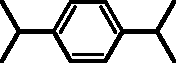
\includegraphics{Figures/Aromatics/diisopropylbenzene.pdf}} & \text{1,4-diisopropylbenzene} & 210.\text{${}^{\circ}$C} & 9.3 \\
 	\hline
 	\raisebox{-.5\height}{\rule{0pt}{18mm}}\raisebox{-.5\height}{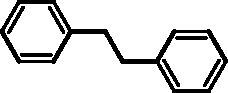
\includegraphics{Figures/Aromatics/bibenzyl.pdf} }& \text{bibenzyl} & 284.\text{${}^{\circ}$C} & 14.2 \\
 	\hline
 	\raisebox{-.5\height}{\rule{0pt}{15mm}}\raisebox{-.5\height}{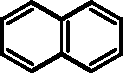
\includegraphics{Figures/Aromatics/naphthalene.pdf}} & \text{naphthalene} & 218.\text{${}^{\circ}$C} & 8.3 \\
 	\hline
 	\raisebox{-.5\height}{\rule{0pt}{15mm}}\raisebox{-.5\height}{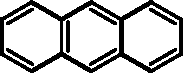
\includegraphics{Figures/Aromatics/anthracene.pdf} }& \text{anthracene} & 340.\text{${}^{\circ}$C} & 7.1 \\
 	\hline
 	\raisebox{-.5\height}{\rule{0pt}{22mm}}\raisebox{-.5\height}{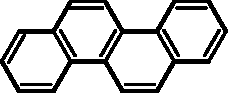
\includegraphics{Figures/Aromatics/chrysene.pdf}} & \text{chrysene} & 448.\text{${}^{\circ}$C} & 3.2 \\
 	\hline
 	\raisebox{-.5\height}{\rule{0pt}{24mm}}\raisebox{-.5\height}{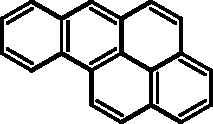
\includegraphics{Figures/Aromatics/benzo[a]pyrene.pdf}}& \text{benzo[\textit{a}]pyrene} & 495.\text{${}^{\circ}$C} & 3.1 \\
 	\hline
\end{tabular}
\end{table}

\subsection{SFC}

The injection system described in Section \ref{sec:SFCInjection} was used to
inject a \SI{0.5}{\micro\litre} volume of the samples. The SFC mobile phase was
neat carbon dioxide at \SI{200}{\bar} inlet pressure. The column consisted of
five HPLC bare silica columns (\SI{150}{\milli\metre} $\times$
\SI{4.6}{\milli\metre}, 3 $\mu$m particles) (Restek, Pinnacle DB Silica)
connected in series.

\subsection{Modulation}

Two modulation periods were used: For the first portion of the chromatogram
\SI{3}{\second} fractions of SFC eluate were collected on the GC column cooled
to a temperature of \SI{-20}{\celsius} or below. The inlet vent was held closed
for \SI{3}{\second} after the the SFC stop valve closed to allow all of the
eluted fraction to be swept onto the column, and then opened for \SI{1}{\second}
to release excess pressure. For the second portion of the chromatogram the same
trapping temperature was used, but the modulation period was increased to
\SI{10}{\second}. This longer trapping period causes a higher increase in inlet
pressure by the eluting carbon dioxide, which required a vent time of
\SI{3}{\second} to release the excess pressure. Under these conditions all the
criteria for comprehensive chromatography (see Section
\ref{sec:SpeedOfAnalysis}) are still met, so the coupling remains comprehensive
throughout the 2D chromatographic run.

\subsection{GC}

The column used in the fast gas chromatograph was a DB-5MS column from J\&W
Scientific Inc, which had a stationary phase comprised of \SI{5}{\percent}
diphenyl, \SI{95}{\percent} di\-meth\-yl\-poly\-si\-lox\-ane. It was
\SI{1}{\metre} long, with an internal diameter of \SI{0.25}{\milli\metre}. The
thickness of the stationary phase was \SI{0.25}{\micro\metre}, and had an
operational temperature range of \SI{-60}{\celsius} to \SI{325}{\celsius} for
isothermal elution, or up to \SI{350}{\celsius} when using temperature
programming.

For every fast GC run the temperature program ramped from \SI{-30}{\celsius} to
\SI{25}{\celsius} at a rate of \SI{8000}{\celsius\per\minute}, and from to
\SI{25}{\celsius} to \SI{350}{\celsius} at a rate of
\SI{2000}{\celsius\per\minute}, where it was held for \SI{2}{s}. After the
temperature program had ended the column was cooled to \SI{-20}{\celsius} again
and the next fraction was collected. Figure \ref{fig:Setpoint_Following}
compares the indicated average temperature of the column with the temperature
program.

\begin{figure}
	\centering
	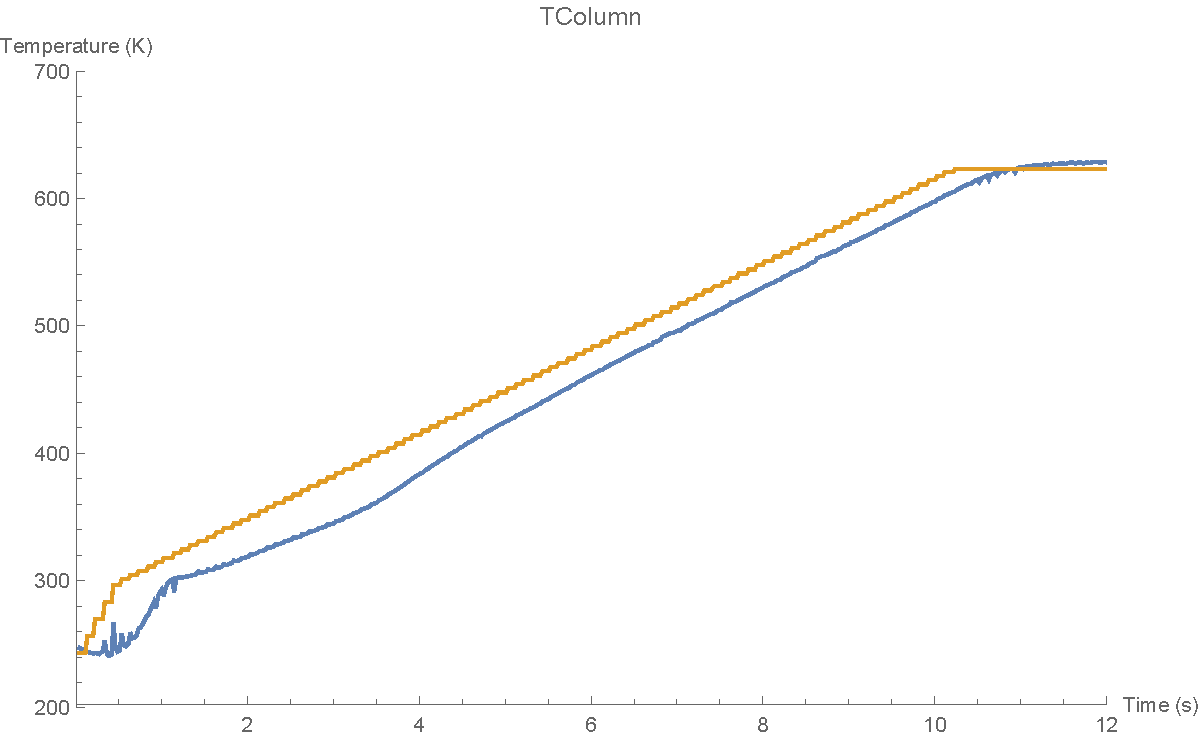
\includegraphics[width=\textwidth]{Figures/Setpoint_Following.pdf}
	\decoRule	
	
\caption[The fidelity of a fast GC temperature program]{A comparison of the
temperature set point and the indicated coaxial heater temperature during a fast
GC run. The orange line shows the intended temperature program and the blue line
shows the actual indicated temperature, as recorded. The ``steps'' in the orange
line are caused by the \SI{100}{\milli\second} period of the control loop.}

	\label{fig:Setpoint_Following} 
\end{figure}

Fast GC chromatograms were obtained by recording the signal of the FID. The oven
temperature of the FID was at \SI{350}{\celsius}. The amplifier gain was set so
that an FID current of \SI{1e-8}{\ampere} gave a \SI{10}{\volt} output signal.
The collected GC chromatograms were used to compile the 2D chromatogram.

\section{Results and discussion}


\begin{figure}
	\centering
	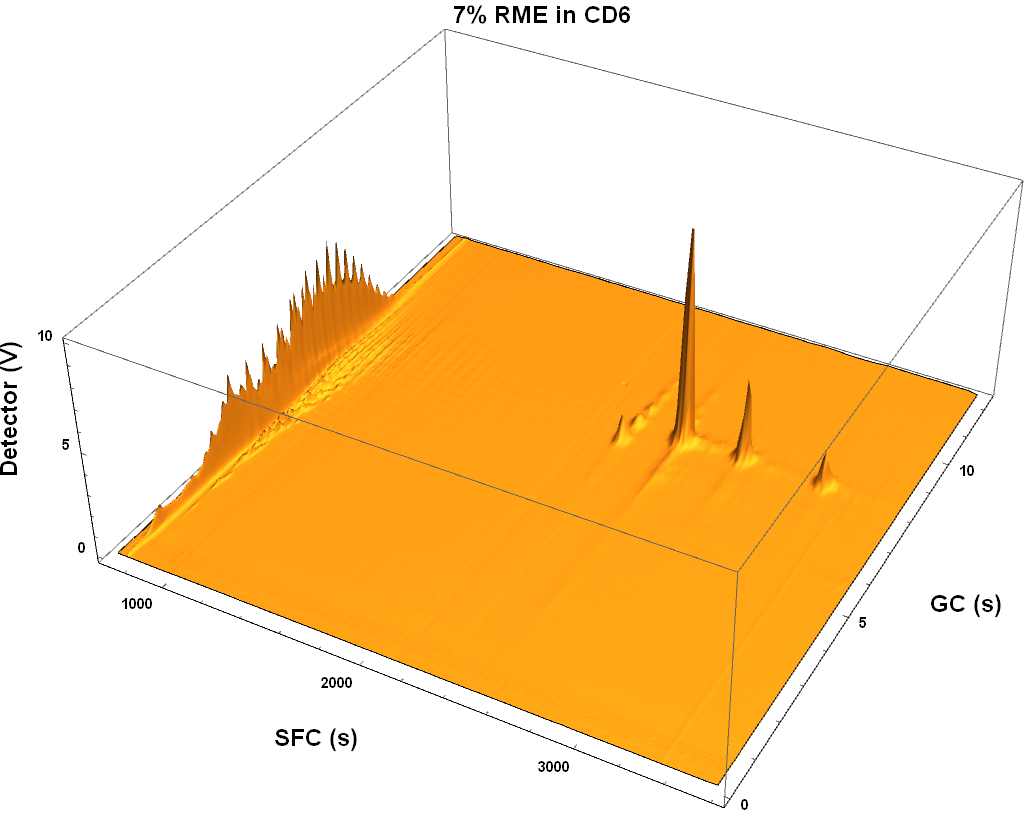
\includegraphics[width=\textwidth]{Figures/PAH_FAMEs.png}
	\decoRule	
	
\caption[Biodiesel separated from petrodiesel.]{A 2D chromatogram of biodiesel
and petrodiesel in a \SI{7}{\percent} blend. The hydrocarbons elute completely
before the first FAME elutes, offering interference-free determination of both.
The chromatogram was compiled from \num{368} 1D fast temperature-programmed GC
chromatograms.}

	\label{fig:PAH_FAMEs} 
\end{figure}




The chromatogram of the biodiesel/petrodiesel blend (Figure \ref{fig:PAH_FAMEs})
shows that the blend was separated into two distinct groups of compounds. At a
\oneD (SFC) retention time of about \SI{780}{\second} the hydrocarbons from the
petrodiesel part of the blend eluted. To those familiar with petrochemical
chromatography the characteristic unresolved complex mixture (``hydrocarbon
hump'') topped by alkane peaks will be instantly recognizable as representing a
petroleum product. (See Figure \ref{fig:HCHump} for an example.)

\begin{figure}
	\centering
	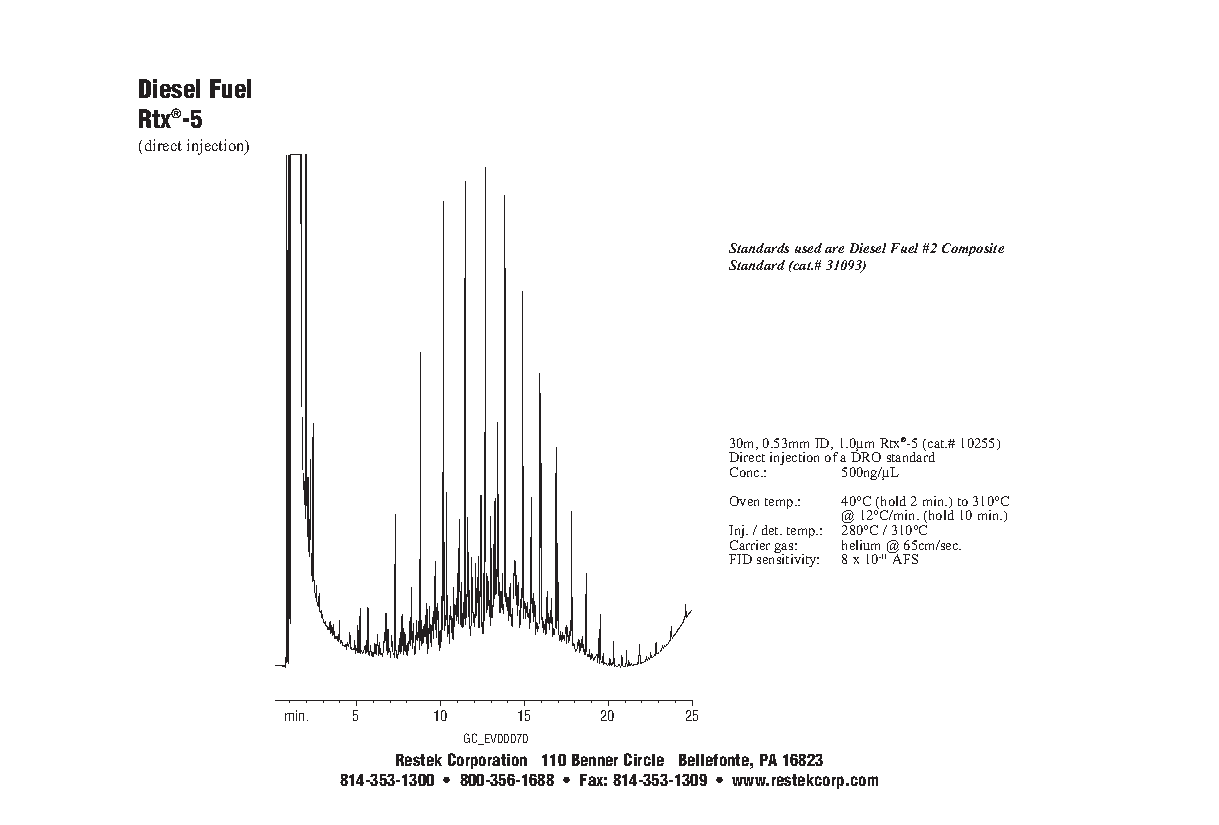
\includegraphics[width=\textwidth]{Figures/hchump.pdf}
	\decoRule	
	
\caption[An example of a petrochemical fuel chromatogram.]{An example of a GC
chromatogram obtained from a petroleum-based diesel fuel sample, showing the
unresolved complex mixture topped by alkane peaks. Restek Searchable
Chromatogram Library, reproduced with permission of Restek Corporation.}
	
	\label{fig:HCHump} 
\end{figure}

At \(^{1}t_{r} \geq \) \SI{2200}{\second} a series of tall peaks represent the
FAMEs, in a pattern that was described in Chapter \ref{Chapter6}: \oneD
separation according to the number of double bonds of the fatty acids, and \twoD
separation according to the chain length of the fatty acids.


\subsection{Aromatic hydrocarbons}

Between \SI{800}{\second} and \SI{1200}{\second} a pattern of small peaks can be
seen in the chromatogram. This portion of the chromatogram is shown magnified in
Figure \ref{fig:Hydrocarbons_Portion}, where individual peaks can clearly be
distinguished.

\begin{figure}
	\centering
	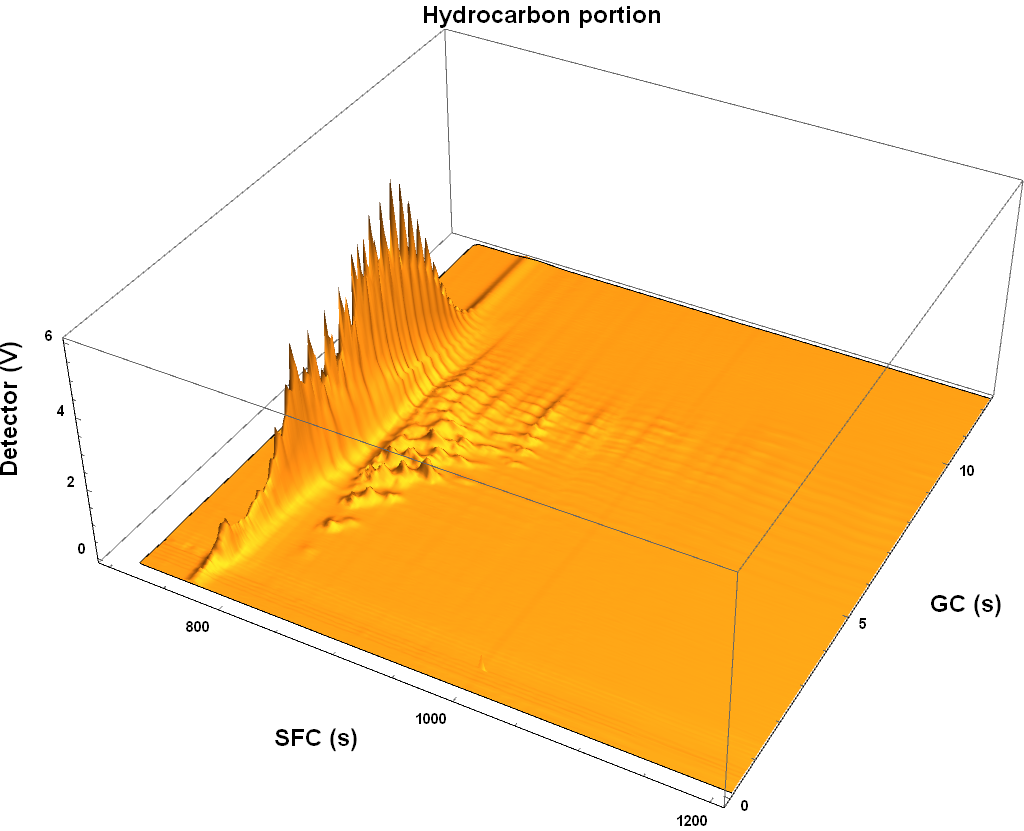
\includegraphics[width=\textwidth]{Figures/Hydrocarbons_Portion.png}
	\decoRule	
	
\caption[Hydrocarbons in RME/diesel blend.]{The portion of the chromatogram of the
\SI{7}{\percent} biodiesel blend that contains the peaks attributed to the hydrocarbons.}
	
	\label{fig:Hydrocarbons_Portion} 
\end{figure}

This result can be compared to the results of the SFC-FID method by integrating
each \twoD GC chromatogram, and plotting these values against their start times.
This creates a virtual SFC chromatogram, which should look similar to 1D SFC
chromatograms. The virtual SFC chromatogram corresponding to Figure
\ref{fig:Hydrocarbons_Portion} is shown in Figure \ref{fig:Virtual_SFC},
compared to an SFC-GC chromatogram taken from the paper on which \std{ASTM 5186}
is based \autocite{DiSanzo1991}. The similarity between the virtual and real
chromatograms suggest that the compounds that elute shortly after the alkanes
are the aromatic hydrocarbons. The virtual chromatogram shows that there is
incomplete separation between the alkanes and the aromatics in the first
dimension, but closer inspection of the 2D chromatogram reveals that there is
complete separation between any aromatic compound and its nearest neighbour
alkane.

\begin{figure}
	\centering
	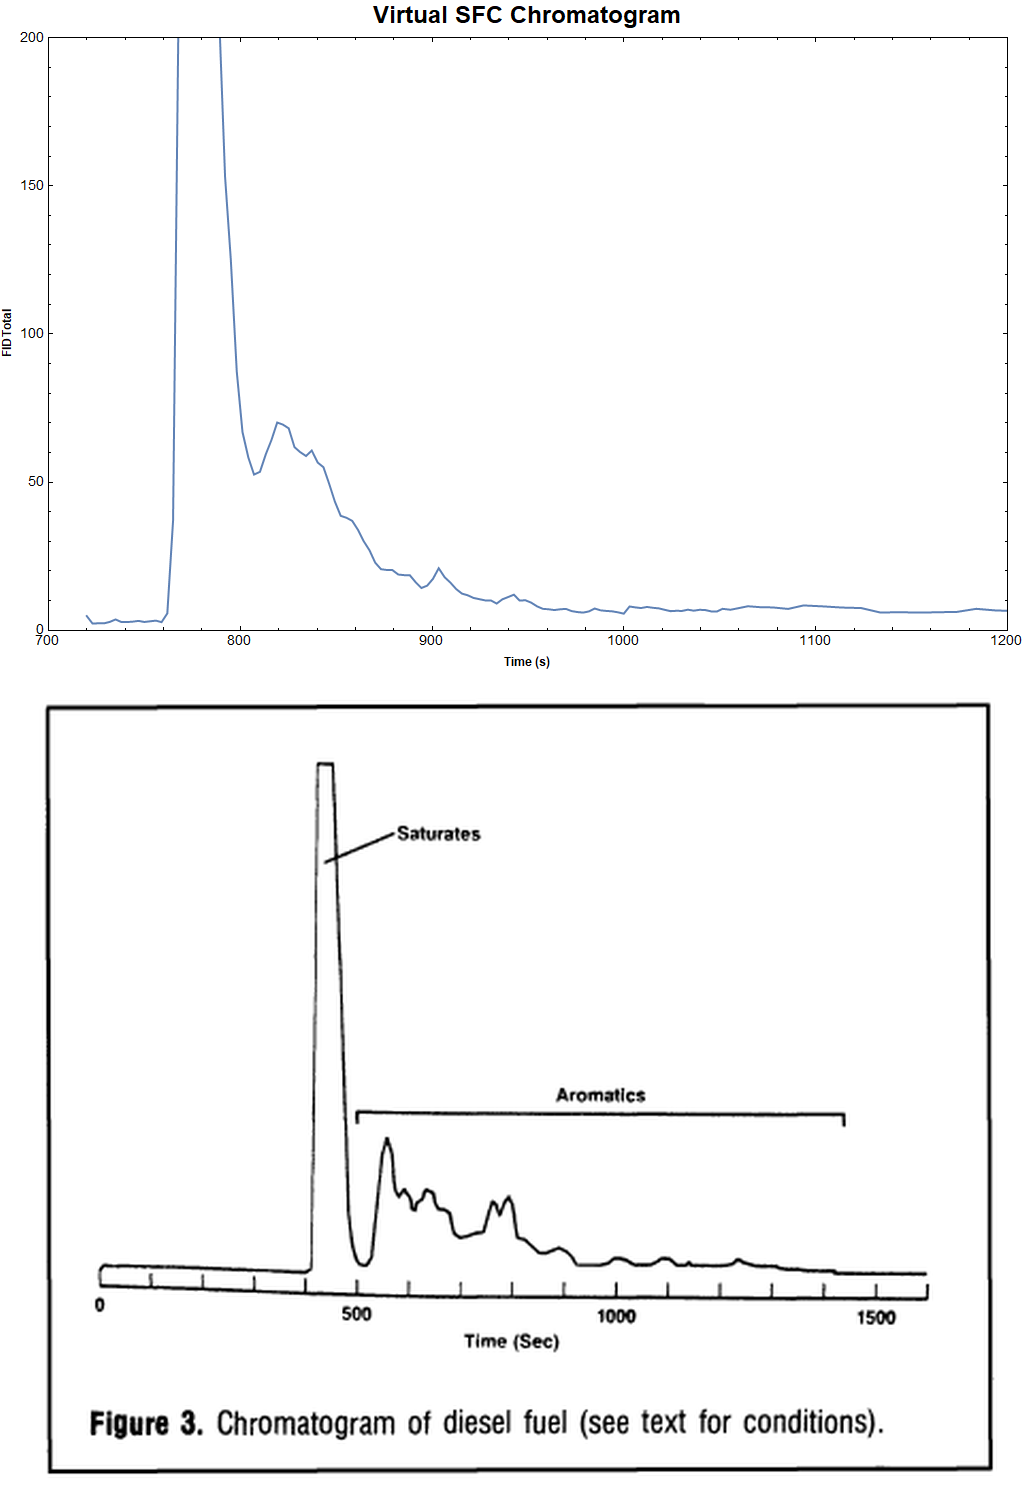
\includegraphics[width=\textwidth]{Figures/VirtualSFC_Compared.png}
	\decoRule	
	
\caption[Comparing SFC-FID and virtual SFC.]{The virtual SFC chromatogram
appears very similar to an SFC-FID chromatogram from literature
\autocite{DiSanzo1991}.}
	
	\label{fig:Virtual_SFC} 
\end{figure}


% \begin{figure}
% 	\centering
% 	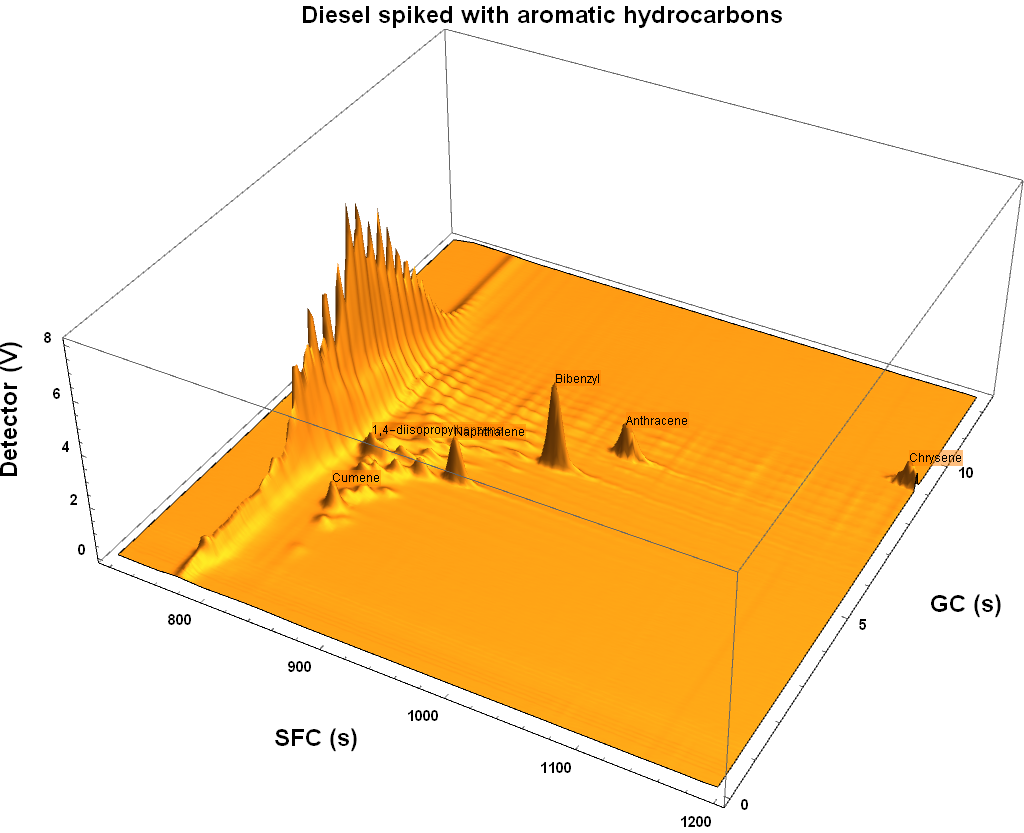
\includegraphics[width=\textwidth]{Figures/Spiked_Diesel.png}
% 	\decoRule	
% 	
% \caption[Spiked diesel ]{A 2D chromatogram of a commercial diesel sample spiked
% with selected aromatic compounds.}
% 
% 	\label{fig:Spiked_Diesel} 
% \end{figure}

Although the identification of peaks of individual aromatic hydrocarbons in the
SFC×GC chromatogram is beyond the scope of this project, injection of the spiked
diesel sample confirms that aromatic compounds elute in this region and shows
that the PAHs in diesel can be clearly separated from the alkanes and
quantified. By comparing the boiling points and relative masses of the spike
compounds, a tentative peak assignment could be made, as shown in Figure
\ref{fig:Spiked_Diesel_Annotated}.

\begin{figure}
	\centering
	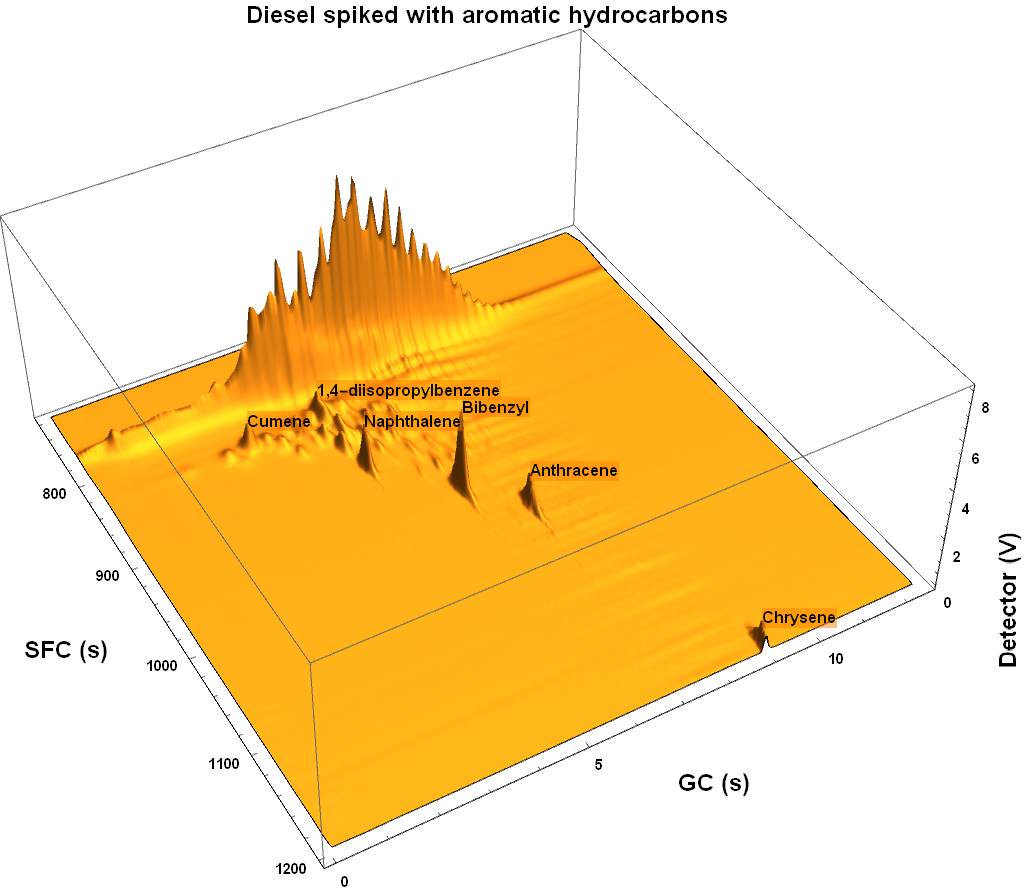
\includegraphics[width=\textwidth]{Figures/Spiked_Diesel_Annotated.png}
	\decoRule	
	
\caption[Peak assignment in spiked diesel sample.]{A 2D chromatogram of a
commercial diesel sample spiked with selected aromatic compounds. Tentative peak
assignments were made using knowledge of the boiling points and relative masses
of the spike compounds.}

	\label{fig:Spiked_Diesel_Annotated} 
\end{figure}

It should be noted that the 5-ring PAH compound benzo[\textit{a}]pyrene that was
included in the spike did not elute in the SFC dimension on this chromatogram.
Its \oneD retention time is still unknown, but broad interfering peaks in
subsequent chromatograms can be attributed to slowly-eluting
benzo[\textit{a}]pyrene shows that it elutes in \twoD without wrap-around, so if
the \oneD run was made longer one would expect its peak to appear in the 2D
chromatogram.

\subsection{FAMEs}

Between the \textsuperscript{1}D retention times of \SI{2200}{\second} and
\SI{3200}{\second} the peaks of the FAMEs are seen, clearly separated by number
of double bonds in the SFC dimension, and by volatility in the GC dimension.
When compared to an SFC×GC chromatogram of FAMEs obtained from canola oil (see
Figure \ref{fig:2DCanola}), the pattern is clearly similar, so the label
``rapeseed methyl ester'' is not incorrect.

\subsection{Adjustable modulation}

Because the SFC is operated in stopped-flow mode, the modulation period is
independent of the fast GC run times. This means that the modulation period can
be adapted during the SFC×GC chromatographic run. Short modulation periods might
be required to preserve resolution obtained in the \oneD separation but in areas
of the chromatogram where there is plenty of resolution the modulation period
can be increased to decrease the run time.

In the chromatogram of the biodiesel blend (Figure \ref{fig:PAH_FAMEs}), the
modulation period was \SI{3}{\second} up to a \oneD retention time of
\SI{1100}{s}. After that the modulation period was increased to
\SI{10}{\second}, which shortened the chromatographic run time. In this
instrument this is the upper limit of the modulation period, and is determined
by the flow of carbon dioxide that the FID flame can tolerate\footnote{If the
flow of carbon dioxide through the column during trapping becomes too high, the
flame is extinguished and the signal disappears. This limitation can be overcome
fairly simply by arranging automatic re-ignition of the flame before the start
of the fast GC run. Then the upper limit of the modulation period depends on the
pressure limit of the GC inlet. This might be determined by mechanical strength,
but experience has also taught that overly high inlet pressures can damage
pressure gauges without any other sign of over-pressure. Alternatively, a
portion of the SFC flow could be split off before it enters the GC inlet.}

\subsubsection{Suspending SFC fraction trapping}

In an extreme version of adjustable modulation, it is also possible to suspend
trapping. This is implemented by opening both the SFC stop valve and the GC
inlet vent and not performing GC runs. The SFC eluate is then swept out of the GC
inlet with no, or minimal, trapping on the GC column. This scheme might be used,
for example, between \(^{1}t_r = 1200\) and \(^{1}t_r = 2200\) of the diesel
blend chromatogram (Figure \ref{fig:PAH_FAMEs}). No peaks of interest elute
during this period, so suspending trapping can save a significant amount of
time.

\subsubsection{Variable GC temperature programs}

Because stopped-flow operation decouples the SFC and the GC, the modulation
period is independent of the GC run time as discussed in the previous section.
But this implies that, conversely,  the GC run time is independent of the
modulation period. This means that the GC fast temperature program can be
adapted to suit the GC separation of the different classes of compounds as
separated by the SFC. For example, in the chromatogram shown in Figure
\ref{fig:PAH_FAMEs} it can be seen that the FAMEs elute in a narrower
temperature range than the hydrocarbons, which suggests that a different
temperature program can be used for optimum separation.

\subsection{Application}

The separation of the compounds found in the \SI{7}{\percent} diesel/biodiesel
blend shows that SFC×GC can be used to investigate the amount of FAMEs and PAHs
in petrodiesel blended with biodiesel without sample pre-treatment or
specialized columns. The intrinsic orthogonality of the separations provides
structured chromatograms which assist with the identification of components and
the ample separation space allows for the addition of suitable internal
standards for reliable qualitative and quantitative analysis by exploiting the
robustness and reliability of the FID. Expensive mass spectrometric detection is
unnecessary.

Being able to determine the biodiesel content of biodiesel blends may prove
useful in at least two scenarios:

The first is in monitoring blending. Biodiesel (essentially a mixture of esters)
is quite polar compared to petrodiesel (essentially a mixture of hydrocarbons).
This means that blending might not be a matter of just pumping the relevant
volumes of the respective fuels into a tank and relying on diffusion to complete
the mixing. Being able to determine the amount of biodiesel in different samples
of a blend will provide assurance that the blend is homogenous and should
perform according to expectations. While such monitoring is perhaps better
performed using a spectroscopic method, SFC×GC can provide information for
calibration, and will of course be invaluable during trouble shooting.

The second application of SFC×GC is in regulating biodiesel content. In some
political environments fuels might be taxed according to their
biologically-derived content, for example to promote agriculture or to meet
carbon emissions targets. Sometimes biological content is simply mandated. Such
incentives and mandates are of course liable to corruption, and therefore it is
necessary to be able to monitor the blending of the fuels. The most
reliable way to differentiate between organic matter derived from biological
sources and organic matter derived from fossil sources is a radiochemical
method, where the content of radioactive \textsuperscript{14}C is determined.
(Organic material from fossil sources contains no \textsuperscript{14}C.) The
technical standard \std{ASTM D6866} provides an approved method. But radiochemical
methods require specialized equipment and trained staff, whereas fuel
laboratories more often have experience with chromatographic techniques and
might find SFC×GC a useful technique to provide evidence that a diesel fuel
blend contains the stated amount of biodiesel.

Apart from demonstrating compliance with regulation, SFC×GC for the
determination of PAHs has potential forensic applications. Oil spills are often
followed by litigation, and methods are required to unambiguously identify
sources of spills. The ratios between different PAHs species is unique to each
crude oil, which transfers to the products distilled from them. Such a ratio
pattern, or PAH \keyword{fingerprint}, can therefore be used to help establish
the source of an oil spill \autocite{Wang2008}. As the results of this chapter
has shown, SFC×GC can be used to generate chromatograms with patterns that could
be used as PAH fingerprints.

\section{Future work}

Previous work has shown that SFC can also separate the alkenes from the alkanes
\autocite{Venter1999}, at least in petrol, and that the resolution can be
improved by cooling the SFC column. Further research along these lines might
reveal that is possible to separate the alkenes from the alkanes in diesel.
While cooling requires more complex instrumentation, the SFC×GC instrument
discussed in this thesis offers two sources of cooling that might be exploited
in such a project: a portion of the coolant used to cool the SFC pump (see
Section \ref{sec:CO2Pump}) can be diverted to cool the column, or any excess
coolant from the cooling cycle of the fast GC can be used to also cool the SFC
column. Alternatively, small solid-state Peltier cooling devices used for
cooling integrated circuits are readily available on the consumer market.

\section{Conclusion}

In the transition to a low-carbon economy that protects and promotes human
dignity and health, the standards set for fuels for internal combustion engines
will continue to evolve. This evolution will pose increasingly challenging
problems to the analytical chemist. While innovation will undoubtedly produce
new analytical instrumentation, the application of SFC×GC to the analysis of
diesel/biodiesel blends shows that is possible to create new, sophisticated
methods of analysis by re-imagining mature, trusted, and reliable analytical
chemistry technologies.

